
\section{Ziel}
In diesem Versuch soll die Ablenkung eines Elektronenstrahls im elektrischen und magnetischen Feld untersucht werden.
\section{Theorie}
\subsection{Aufbau einer Kathodenstrahlröhre}
Die Kathodenstrahlröhre besteht aus drei Teilen: der sogenannten Elektronenkanone, einem Ablenk- und einem Nachweissystem.
Die Elektronenkanone erzeugt freie Elektronen durch Glühemission.
Die dabei erhitzte Kathode wird von einem Wehnelt-Zylinder umgeben, der in Abbildung \ref{fig:WZ} dargestellt wird.
\begin{figure}[H]
  \centering
  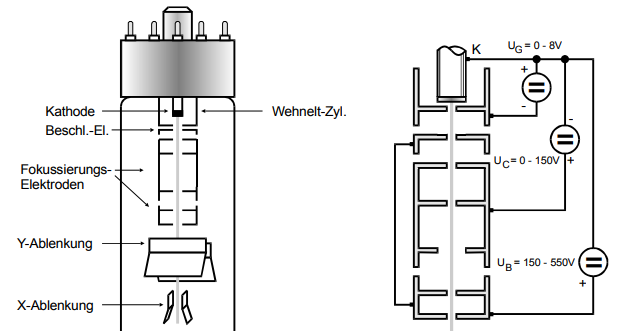
\includegraphics[width=\linewidth-100pt,height=\textheight-100pt,keepaspectratio]{Text/Bilder/Kathodenstrahlroehre.png}
  \caption{Querschnitt durch eine Kathodenstrahlröhre und die Beschaltung ihrer „Elektronenkanone" \cite[82]{sample}}
  \label{fig:WZ}
\end{figure}
Aufgrund der Potentialdifferenz zwischen Kathode und dem Wehnelt-Zylinder, steuert letzterer die Intensität des Elektronenstrahls.
Zusätzlich befindet sich vor diesem eine Elektrode mit hohen positiven Potential gegenüber der Kathode. Diese beschleunigt die Elektronen auf die Geschwindigkeit
\begin{equation}
  v=\sqrt{\frac{2 e_0 U_B}{m}} \text{.} \label{eqn:vnk}
\end{equation}
Nachdem die Elektronen auf diese Geschwindigkeit beschleunigt wurden, werden sie durch sich an den Seiten befindenden Elektroden, den Elektronenlinsen, abgelenkt und fokussiert.
Bevor die Elektronen jedoch den Leuchtschirm erreichen, passieren sie das Ablenksystem. Dieses besteht aus zwei je paralellen Plattenpaaren, in denen der Elektronenstrahl durch elektrische Felder in X- bzw Y-Richtung
abgelenkt wird. Dies wird in \ref{sec:AiE} näher erläutert.
Danach treffen die Elektronen auf den Leuchtschirm, auf dem ihre Position durch emittierte Lichtquanten sichtbar gemacht wird. Zur Emission kommt es durch Anregung der Aktivatorzentren im Schirm, d.h. Störstellen im Gitter
des Materials. Damit der Schirm elektrisch neutral bleibt, ist dieser mit der Beschleunigungselektrode verbunden.
\subsection{Ablenkung im E-Feld} \label{sec:AiE}
Bei einem Plattenpaar mit Abstand $d$ und Länge $l$ kann für den Fall $d \ll l$ das Feld zwischen den Platten mit
\begin{equation}
E=\frac{U_d}{d}
\end{equation}
als konstant genähert werden. Das Elektron erfährt dann die Kraft
\begin{equation}
  F= \left | \vec{E}\cdot e_0 \right | = e_0 \cdot \frac{U_d}{d}
\end{equation}
über einen Zeitraum $\Delta t$. Damit wird es, wie in Abbildung \ref{fig:SidK} zu sehen ist, konstant in y-Richtung abgelenkt.
Da $F$ konstant ist, gilt mit $v=a_y \cdot \Delta t$ und $a_y = F/m_0$ :
\begin{equation}
  v_y=\frac{e_0}{m_0}\frac{U_d}{d}\Delta t \label{eqn:bla}
\end{equation}
Aus Abbildung \ref{fig:SidK} lassen sich zusätzlich die Zusammenhänge $\Delta t =\frac{p}{v_z}$ und $\theta=\frac{v_y}{v_z}$
entnehmen, womit \eqref{eqn:bla} umgeschrieben werden kann zu
\begin{equation}
  v_y=\frac{e_0}{m_0} \frac{U_d}{d} \frac{p}{v_z} \text{.}
\end{equation}
Damit gilt die Verschiebung
\begin{equation}
  D=\frac{e_0}{m_0} \frac{U_d}{d} \frac{p}{(v_z)^2}L =\frac{p}{2d}\frac{U_d}{U_B}L \text{.}
\end{equation}
\begin{figure}
  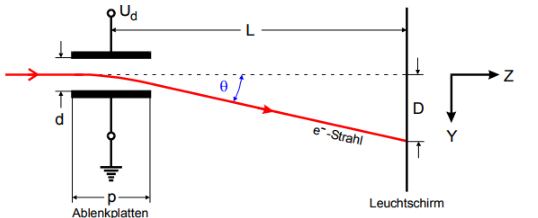
\includegraphics[width=\linewidth-100pt,height=\textheight-100pt,keepaspectratio]{Text/Bilder/Ablenkplatten.png}
  \caption{Strahlablenkung in der Kathodenstrahlröhre\cite[83]{sample}.}
  \label{fig:SidK}
\end{figure}
%Aus diesem Zusammenhang ergibt sich auch, dass für eine hohe Ablenkempfindlichkeit $L$
%und $p$ groß sein müssen, währenddessen $U_B$ klein sein muss. In diesem Fall könnten jedoch
%nur niederfequente Spannungen untersucht werden, da die Flugzeit $\Delta t$ klein gegen die
%Periodendauer von $U$ sein muss.
%Bei hochfrequenten Wechselspannungen muss dagegen $p$ klein und $U_b$ groß sein.

\subsection{Kathodenstrahl-Oszillographen}
Wird an den Platten, die den Elektronenstrahl in X-Richtung ablenken, eine Wechsel-
spannung und an das andere Plattenpaar die zu untersuchende Spannung angebracht,
so kann eine Kathodenstrahlröhre zu einem Kathodenstrahl-Oszillographen erweitert
werden. Diese erlaubt es, die Zeitabhängigkeit von Wechselspannungen darzustellen. Sind
die beiden Spannungen im passenden Verhältnis zueinander, so zeichnet sich der zeitliche
Verlauf am Laufschirm ab. Es soll gelten:
\begin{align}
  n \cdot v_\text{Sä} = m \cdot v_\text{Sig} && \text{n, m} \in \mathds{N}
\end{align}

\subsection{ Ablenkung im B-Feld}
Bewegt sich eine Ladung $q$ mit einer Geschwindigkeit $v$ verschieden von $0$ in einem magnetischen statt einem elektrischen Feld , so wirkt auf
dieses die Lorentzkraft:
\begin{equation}
  \vec{F}=q \cdot \vec{v} \times \vec{B}
\end{equation}
Im Fall $\vec{v} \bot \vec{B}$  gilt für ein Elektron:
\begin{equation}
  F_L= e_0 \cdot v \cdot B
\end{equation}

Wie in Abbildung \ref{fig:WDM} zu sehen ist, bewegen sich die Elektronen mit der in \eqref{eqn:vnk} gegebenen
Geschwindigkeit geradlinig, bis sie bis sie durch die Lorentzkraft auf eine Kreisbahn
geraten, womit diese der Zentripetalkraft $F = \frac{mv^2}{r}$
entspricht. Damit gilt für den Radius:
\begin{equation}
  r=\frac{m_0 v_0}{e_0 B}
\end{equation}
\begin{figure}[H]
  \centering
  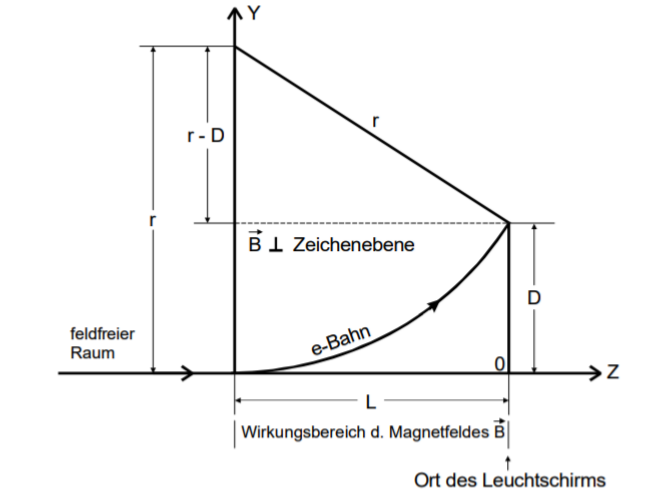
\includegraphics{Text/Bilder/WDM.png}
  \caption{ Skizze zur Ableitung einer Beziehung zwischen L, D und r \cite[89]{sample2}.}
  \label{fig:WDM}
\end{figure}
Für die in \ref{fig:WDM} zu sehende Konstallation folgt dann aus geometrischen Überlegung und \eqref{eqn:vnk} der
Zusammenhang
\begin{equation}
  \frac{D}{D^2+L^2}=\frac{1}{8U_B}\sqrt{\frac{e_0}{m_o}}B \text{.}
\end{equation}
